% Created by tikzDevice version 0.12.3.1 on 2021-05-25 12:20:32
% !TEX encoding = UTF-8 Unicode
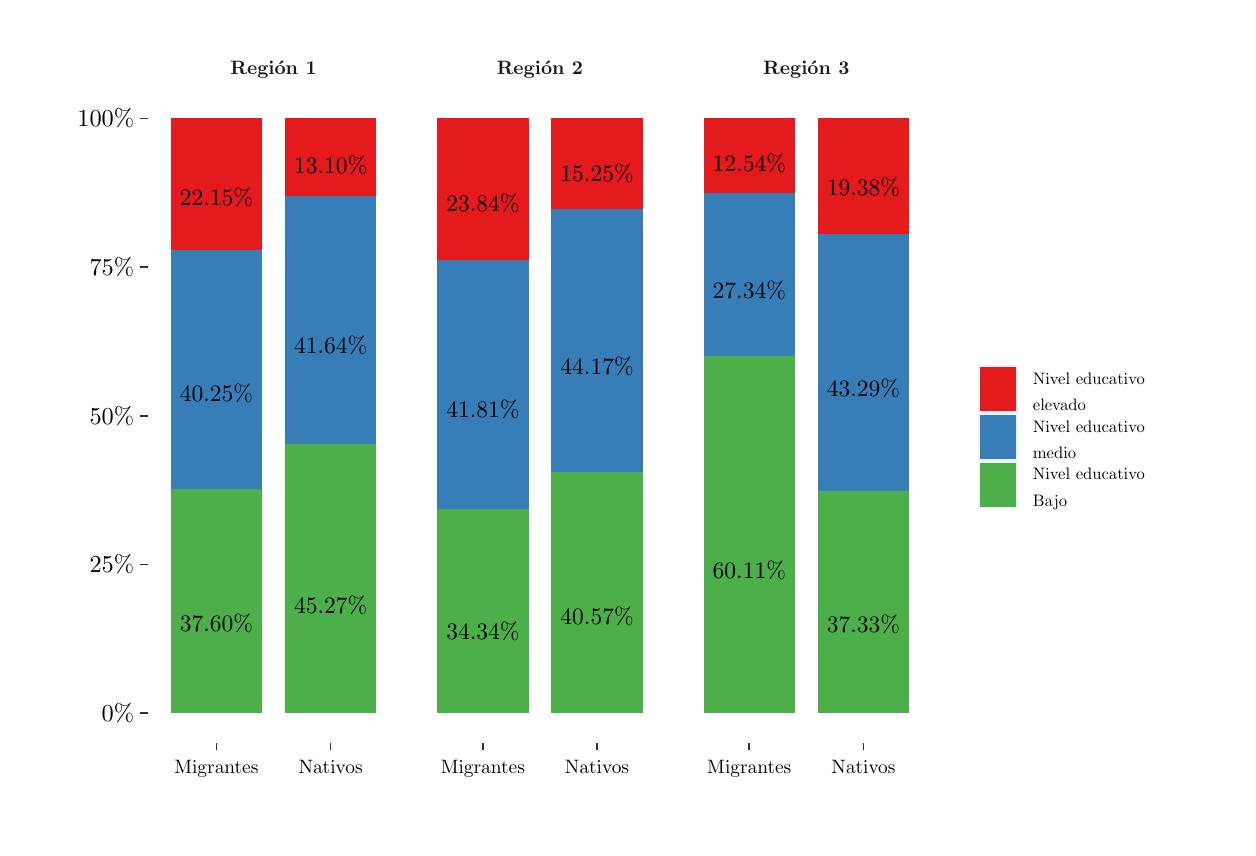
\begin{tikzpicture}[x=1pt,y=1pt]
\definecolor{fillColor}{RGB}{255,255,255}
\path[use as bounding box,fill=fillColor,fill opacity=0.00] (0,0) rectangle (433.62,289.08);
\begin{scope}
\path[clip] (  0.00,  0.00) rectangle (433.62,289.08);
\definecolor{drawColor}{RGB}{255,255,255}
\definecolor{fillColor}{RGB}{255,255,255}

\path[draw=drawColor,line width= 0.6pt,line join=round,line cap=round,fill=fillColor] (  0.00,  0.00) rectangle (433.62,289.08);
\end{scope}
\begin{scope}
\path[clip] ( 43.44, 30.69) rectangle (134.22,267.01);
\definecolor{drawColor}{RGB}{255,255,255}

\path[draw=drawColor,line width= 0.3pt,line join=round] ( 43.44, 68.28) --
	(134.22, 68.28);

\path[draw=drawColor,line width= 0.3pt,line join=round] ( 43.44,121.99) --
	(134.22,121.99);

\path[draw=drawColor,line width= 0.3pt,line join=round] ( 43.44,175.70) --
	(134.22,175.70);

\path[draw=drawColor,line width= 0.3pt,line join=round] ( 43.44,229.41) --
	(134.22,229.41);

\path[draw=drawColor,line width= 0.6pt,line join=round] ( 43.44, 41.43) --
	(134.22, 41.43);

\path[draw=drawColor,line width= 0.6pt,line join=round] ( 43.44, 95.14) --
	(134.22, 95.14);

\path[draw=drawColor,line width= 0.6pt,line join=round] ( 43.44,148.85) --
	(134.22,148.85);

\path[draw=drawColor,line width= 0.6pt,line join=round] ( 43.44,202.56) --
	(134.22,202.56);

\path[draw=drawColor,line width= 0.6pt,line join=round] ( 43.44,256.27) --
	(134.22,256.27);

\path[draw=drawColor,line width= 0.6pt,line join=round] ( 68.20, 30.69) --
	( 68.20,267.01);

\path[draw=drawColor,line width= 0.6pt,line join=round] (109.46, 30.69) --
	(109.46,267.01);
\definecolor{fillColor}{RGB}{228,26,28}

\path[fill=fillColor] ( 51.70,208.68) rectangle ( 84.71,256.27);
\definecolor{fillColor}{RGB}{55,126,184}

\path[fill=fillColor] ( 51.70,122.21) rectangle ( 84.71,208.68);
\definecolor{fillColor}{RGB}{77,175,74}

\path[fill=fillColor] ( 51.70, 41.43) rectangle ( 84.71,122.21);
\definecolor{fillColor}{RGB}{228,26,28}

\path[fill=fillColor] ( 92.96,228.13) rectangle (125.97,256.27);
\definecolor{fillColor}{RGB}{55,126,184}

\path[fill=fillColor] ( 92.96,138.68) rectangle (125.97,228.13);
\definecolor{fillColor}{RGB}{77,175,74}

\path[fill=fillColor] ( 92.96, 41.43) rectangle (125.97,138.68);
\definecolor{drawColor}{RGB}{0,0,0}

\node[text=drawColor,anchor=base,inner sep=0pt, outer sep=0pt, scale=  0.85] at ( 68.20,224.78) {22.15{\%}};

\node[text=drawColor,anchor=base,inner sep=0pt, outer sep=0pt, scale=  0.85] at ( 68.20,153.86) {40.25{\%}};

\node[text=drawColor,anchor=base,inner sep=0pt, outer sep=0pt, scale=  0.85] at ( 68.20, 70.80) {37.60{\%}};

\node[text=drawColor,anchor=base,inner sep=0pt, outer sep=0pt, scale=  0.85] at (109.46,236.44) {13.10{\%}};

\node[text=drawColor,anchor=base,inner sep=0pt, outer sep=0pt, scale=  0.85] at (109.46,171.52) {41.64{\%}};

\node[text=drawColor,anchor=base,inner sep=0pt, outer sep=0pt, scale=  0.85] at (109.46, 77.39) {45.27{\%}};
\end{scope}
\begin{scope}
\path[clip] (139.72, 30.69) rectangle (230.50,267.01);
\definecolor{drawColor}{RGB}{255,255,255}

\path[draw=drawColor,line width= 0.3pt,line join=round] (139.72, 68.28) --
	(230.50, 68.28);

\path[draw=drawColor,line width= 0.3pt,line join=round] (139.72,121.99) --
	(230.50,121.99);

\path[draw=drawColor,line width= 0.3pt,line join=round] (139.72,175.70) --
	(230.50,175.70);

\path[draw=drawColor,line width= 0.3pt,line join=round] (139.72,229.41) --
	(230.50,229.41);

\path[draw=drawColor,line width= 0.6pt,line join=round] (139.72, 41.43) --
	(230.50, 41.43);

\path[draw=drawColor,line width= 0.6pt,line join=round] (139.72, 95.14) --
	(230.50, 95.14);

\path[draw=drawColor,line width= 0.6pt,line join=round] (139.72,148.85) --
	(230.50,148.85);

\path[draw=drawColor,line width= 0.6pt,line join=round] (139.72,202.56) --
	(230.50,202.56);

\path[draw=drawColor,line width= 0.6pt,line join=round] (139.72,256.27) --
	(230.50,256.27);

\path[draw=drawColor,line width= 0.6pt,line join=round] (164.48, 30.69) --
	(164.48,267.01);

\path[draw=drawColor,line width= 0.6pt,line join=round] (205.74, 30.69) --
	(205.74,267.01);
\definecolor{fillColor}{RGB}{228,26,28}

\path[fill=fillColor] (147.97,205.04) rectangle (180.99,256.27);
\definecolor{fillColor}{RGB}{55,126,184}

\path[fill=fillColor] (147.97,115.21) rectangle (180.99,205.04);
\definecolor{fillColor}{RGB}{77,175,74}

\path[fill=fillColor] (147.97, 41.43) rectangle (180.99,115.21);
\definecolor{fillColor}{RGB}{228,26,28}

\path[fill=fillColor] (189.24,223.50) rectangle (222.25,256.27);
\definecolor{fillColor}{RGB}{55,126,184}

\path[fill=fillColor] (189.24,128.59) rectangle (222.25,223.50);
\definecolor{fillColor}{RGB}{77,175,74}

\path[fill=fillColor] (189.24, 41.43) rectangle (222.25,128.59);
\definecolor{drawColor}{RGB}{0,0,0}

\node[text=drawColor,anchor=base,inner sep=0pt, outer sep=0pt, scale=  0.85] at (164.48,222.59) {23.84{\%}};

\node[text=drawColor,anchor=base,inner sep=0pt, outer sep=0pt, scale=  0.85] at (164.48,148.20) {41.81{\%}};

\node[text=drawColor,anchor=base,inner sep=0pt, outer sep=0pt, scale=  0.85] at (164.48, 68.00) {34.34{\%}};

\node[text=drawColor,anchor=base,inner sep=0pt, outer sep=0pt, scale=  0.85] at (205.74,233.66) {15.25{\%}};

\node[text=drawColor,anchor=base,inner sep=0pt, outer sep=0pt, scale=  0.85] at (205.74,163.62) {44.17{\%}};

\node[text=drawColor,anchor=base,inner sep=0pt, outer sep=0pt, scale=  0.85] at (205.74, 73.36) {40.57{\%}};
\end{scope}
\begin{scope}
\path[clip] (236.00, 30.69) rectangle (326.78,267.01);
\definecolor{drawColor}{RGB}{255,255,255}

\path[draw=drawColor,line width= 0.3pt,line join=round] (236.00, 68.28) --
	(326.78, 68.28);

\path[draw=drawColor,line width= 0.3pt,line join=round] (236.00,121.99) --
	(326.78,121.99);

\path[draw=drawColor,line width= 0.3pt,line join=round] (236.00,175.70) --
	(326.78,175.70);

\path[draw=drawColor,line width= 0.3pt,line join=round] (236.00,229.41) --
	(326.78,229.41);

\path[draw=drawColor,line width= 0.6pt,line join=round] (236.00, 41.43) --
	(326.78, 41.43);

\path[draw=drawColor,line width= 0.6pt,line join=round] (236.00, 95.14) --
	(326.78, 95.14);

\path[draw=drawColor,line width= 0.6pt,line join=round] (236.00,148.85) --
	(326.78,148.85);

\path[draw=drawColor,line width= 0.6pt,line join=round] (236.00,202.56) --
	(326.78,202.56);

\path[draw=drawColor,line width= 0.6pt,line join=round] (236.00,256.27) --
	(326.78,256.27);

\path[draw=drawColor,line width= 0.6pt,line join=round] (260.76, 30.69) --
	(260.76,267.01);

\path[draw=drawColor,line width= 0.6pt,line join=round] (302.02, 30.69) --
	(302.02,267.01);
\definecolor{fillColor}{RGB}{228,26,28}

\path[fill=fillColor] (244.25,229.32) rectangle (277.26,256.27);
\definecolor{fillColor}{RGB}{55,126,184}

\path[fill=fillColor] (244.25,170.57) rectangle (277.26,229.32);
\definecolor{fillColor}{RGB}{77,175,74}

\path[fill=fillColor] (244.25, 41.43) rectangle (277.26,170.57);
\definecolor{fillColor}{RGB}{228,26,28}

\path[fill=fillColor] (285.52,214.63) rectangle (318.53,256.27);
\definecolor{fillColor}{RGB}{55,126,184}

\path[fill=fillColor] (285.52,121.62) rectangle (318.53,214.63);
\definecolor{fillColor}{RGB}{77,175,74}

\path[fill=fillColor] (285.52, 41.43) rectangle (318.53,121.62);
\definecolor{drawColor}{RGB}{0,0,0}

\node[text=drawColor,anchor=base,inner sep=0pt, outer sep=0pt, scale=  0.85] at (260.76,237.16) {12.54{\%}};

\node[text=drawColor,anchor=base,inner sep=0pt, outer sep=0pt, scale=  0.85] at (260.76,191.13) {27.34{\%}};

\node[text=drawColor,anchor=base,inner sep=0pt, outer sep=0pt, scale=  0.85] at (260.76, 90.15) {60.11{\%}};

\node[text=drawColor,anchor=base,inner sep=0pt, outer sep=0pt, scale=  0.85] at (302.02,228.35) {19.38{\%}};

\node[text=drawColor,anchor=base,inner sep=0pt, outer sep=0pt, scale=  0.85] at (302.02,155.89) {43.29{\%}};

\node[text=drawColor,anchor=base,inner sep=0pt, outer sep=0pt, scale=  0.85] at (302.02, 70.57) {37.33{\%}};
\end{scope}
\begin{scope}
\path[clip] ( 43.44,267.01) rectangle (134.22,283.58);
\definecolor{drawColor}{gray}{0.10}

\node[text=drawColor,anchor=base,inner sep=0pt, outer sep=0pt, scale=  0.70] at ( 88.83,272.26) {\textbf{Región 1}};
\end{scope}
\begin{scope}
\path[clip] (139.72,267.01) rectangle (230.50,283.58);
\definecolor{drawColor}{gray}{0.10}

\node[text=drawColor,anchor=base,inner sep=0pt, outer sep=0pt, scale=  0.70] at (185.11,272.26) {\textbf{Región 2}};
\end{scope}
\begin{scope}
\path[clip] (236.00,267.01) rectangle (326.78,283.58);
\definecolor{drawColor}{gray}{0.10}

\node[text=drawColor,anchor=base,inner sep=0pt, outer sep=0pt, scale=  0.70] at (281.39,272.26) {\textbf{Región 3}};
\end{scope}
\begin{scope}
\path[clip] (  0.00,  0.00) rectangle (433.62,289.08);
\definecolor{drawColor}{gray}{0.20}

\path[draw=drawColor,line width= 0.6pt,line join=round] ( 68.20, 27.94) --
	( 68.20, 30.69);

\path[draw=drawColor,line width= 0.6pt,line join=round] (109.46, 27.94) --
	(109.46, 30.69);
\end{scope}
\begin{scope}
\path[clip] (  0.00,  0.00) rectangle (433.62,289.08);
\definecolor{drawColor}{RGB}{0,0,0}

\node[text=drawColor,anchor=base,inner sep=0pt, outer sep=0pt, scale=  0.70] at ( 68.20, 19.68) {Migrantes};

\node[text=drawColor,anchor=base,inner sep=0pt, outer sep=0pt, scale=  0.70] at (109.46, 19.68) {Nativos};
\end{scope}
\begin{scope}
\path[clip] (  0.00,  0.00) rectangle (433.62,289.08);
\definecolor{drawColor}{gray}{0.20}

\path[draw=drawColor,line width= 0.6pt,line join=round] (164.48, 27.94) --
	(164.48, 30.69);

\path[draw=drawColor,line width= 0.6pt,line join=round] (205.74, 27.94) --
	(205.74, 30.69);
\end{scope}
\begin{scope}
\path[clip] (  0.00,  0.00) rectangle (433.62,289.08);
\definecolor{drawColor}{RGB}{0,0,0}

\node[text=drawColor,anchor=base,inner sep=0pt, outer sep=0pt, scale=  0.70] at (164.48, 19.68) {Migrantes};

\node[text=drawColor,anchor=base,inner sep=0pt, outer sep=0pt, scale=  0.70] at (205.74, 19.68) {Nativos};
\end{scope}
\begin{scope}
\path[clip] (  0.00,  0.00) rectangle (433.62,289.08);
\definecolor{drawColor}{gray}{0.20}

\path[draw=drawColor,line width= 0.6pt,line join=round] (260.76, 27.94) --
	(260.76, 30.69);

\path[draw=drawColor,line width= 0.6pt,line join=round] (302.02, 27.94) --
	(302.02, 30.69);
\end{scope}
\begin{scope}
\path[clip] (  0.00,  0.00) rectangle (433.62,289.08);
\definecolor{drawColor}{RGB}{0,0,0}

\node[text=drawColor,anchor=base,inner sep=0pt, outer sep=0pt, scale=  0.70] at (260.76, 19.68) {Migrantes};

\node[text=drawColor,anchor=base,inner sep=0pt, outer sep=0pt, scale=  0.70] at (302.02, 19.68) {Nativos};
\end{scope}
\begin{scope}
\path[clip] (  0.00,  0.00) rectangle (433.62,289.08);
\definecolor{drawColor}{RGB}{0,0,0}

\node[text=drawColor,anchor=base east,inner sep=0pt, outer sep=0pt, scale=  0.88] at ( 38.49, 38.40) {0{\%}};

\node[text=drawColor,anchor=base east,inner sep=0pt, outer sep=0pt, scale=  0.88] at ( 38.49, 92.11) {25{\%}};

\node[text=drawColor,anchor=base east,inner sep=0pt, outer sep=0pt, scale=  0.88] at ( 38.49,145.82) {50{\%}};

\node[text=drawColor,anchor=base east,inner sep=0pt, outer sep=0pt, scale=  0.88] at ( 38.49,199.53) {75{\%}};

\node[text=drawColor,anchor=base east,inner sep=0pt, outer sep=0pt, scale=  0.88] at ( 38.49,253.24) {100{\%}};
\end{scope}
\begin{scope}
\path[clip] (  0.00,  0.00) rectangle (433.62,289.08);
\definecolor{drawColor}{gray}{0.20}

\path[draw=drawColor,line width= 0.6pt,line join=round] ( 40.69, 41.43) --
	( 43.44, 41.43);

\path[draw=drawColor,line width= 0.6pt,line join=round] ( 40.69, 95.14) --
	( 43.44, 95.14);

\path[draw=drawColor,line width= 0.6pt,line join=round] ( 40.69,148.85) --
	( 43.44,148.85);

\path[draw=drawColor,line width= 0.6pt,line join=round] ( 40.69,202.56) --
	( 43.44,202.56);

\path[draw=drawColor,line width= 0.6pt,line join=round] ( 40.69,256.27) --
	( 43.44,256.27);
\end{scope}
\begin{scope}
\path[clip] (  0.00,  0.00) rectangle (433.62,289.08);
\definecolor{fillColor}{RGB}{255,255,255}

\path[fill=fillColor] (337.78,109.83) rectangle (428.12,187.87);
\end{scope}
\begin{scope}
\path[clip] (  0.00,  0.00) rectangle (433.62,289.08);
\definecolor{fillColor}{gray}{0.95}

\path[fill=fillColor] (343.28,149.88) rectangle (357.73,167.15);
\end{scope}
\begin{scope}
\path[clip] (  0.00,  0.00) rectangle (433.62,289.08);
\definecolor{fillColor}{RGB}{228,26,28}

\path[fill=fillColor] (343.99,150.59) rectangle (357.02,166.44);
\end{scope}
\begin{scope}
\path[clip] (  0.00,  0.00) rectangle (433.62,289.08);
\definecolor{fillColor}{gray}{0.95}

\path[fill=fillColor] (343.28,132.60) rectangle (357.73,149.88);
\end{scope}
\begin{scope}
\path[clip] (  0.00,  0.00) rectangle (433.62,289.08);
\definecolor{fillColor}{RGB}{55,126,184}

\path[fill=fillColor] (343.99,133.31) rectangle (357.02,149.17);
\end{scope}
\begin{scope}
\path[clip] (  0.00,  0.00) rectangle (433.62,289.08);
\definecolor{fillColor}{gray}{0.95}

\path[fill=fillColor] (343.28,115.33) rectangle (357.73,132.60);
\end{scope}
\begin{scope}
\path[clip] (  0.00,  0.00) rectangle (433.62,289.08);
\definecolor{fillColor}{RGB}{77,175,74}

\path[fill=fillColor] (343.99,116.04) rectangle (357.02,131.89);
\end{scope}
\begin{scope}
\path[clip] (  0.00,  0.00) rectangle (433.62,289.08);
\definecolor{drawColor}{RGB}{0,0,0}

\node[text=drawColor,anchor=base west,inner sep=0pt, outer sep=0pt, scale=  0.60] at (363.23,160.24) {Nivel educativo};

\node[text=drawColor,anchor=base west,inner sep=0pt, outer sep=0pt, scale=  0.60] at (363.23,150.73) {elevado};
\end{scope}
\begin{scope}
\path[clip] (  0.00,  0.00) rectangle (433.62,289.08);
\definecolor{drawColor}{RGB}{0,0,0}

\node[text=drawColor,anchor=base west,inner sep=0pt, outer sep=0pt, scale=  0.60] at (363.23,142.96) {Nivel educativo};

\node[text=drawColor,anchor=base west,inner sep=0pt, outer sep=0pt, scale=  0.60] at (363.23,133.46) {medio};
\end{scope}
\begin{scope}
\path[clip] (  0.00,  0.00) rectangle (433.62,289.08);
\definecolor{drawColor}{RGB}{0,0,0}

\node[text=drawColor,anchor=base west,inner sep=0pt, outer sep=0pt, scale=  0.60] at (363.23,125.69) {Nivel educativo};

\node[text=drawColor,anchor=base west,inner sep=0pt, outer sep=0pt, scale=  0.60] at (363.23,116.18) {Bajo};
\end{scope}
\end{tikzpicture}
